\textit{Activity Model} é estruturado sobre uma linguagem de descrição conhecido por \textit{ACTIVITY-DL}. Um dos elementos dessa linguagem é baseado na álgebra de Allen's que tem como por finalidade definir raciocínios temporais \cite{allenalgebric}. 
As relações definidas por essa álgebra é dada por; 

\begin{enumerate}
	\item $X < Y$ onde $X$: ocorre antes de $Y$ 
	\item $X m Y$,$Y mi X$: $X$ encontra $Y$
	\item $X o Y$, $X oi Y$: $X$ sobrepõem a $Y$
	\item $X s Y$, $Y si X$: $X$ começa $Y$
	\item $X d Y$, $Y di X$: $X$ ocorre durante $Y$	  
	\item $X f Y$, $Y fi X$: $X$ termina junto com $Y$	  	
	\item $X = Y$ $X$ é igual a $Y$	  		
\end{enumerate}

A \textit{Activity Model} define construtores que são semanticamente equivalente a certos operadores da álgebra de Allen's. Esses construtores (atuantes sobre atividades) são definidos pela tabela \ref{acticonstruct}

\begin{table}[H]
\centering
\begin{tabular}{|l|l|l|}
\hline
Construtor & Nome         & Relações de Allen \\ \hline
IND        & Independent  & $A \{ <,>,m,mi,o,oi,s,si,d,di,f,fi,= \} B$\\ \hline
SEQ        & Sequential   & $A \{ <,>,m,mi \} B$\\ \hline
SEQ-ORD    & Ordered      & $A \{ <,>,m \} B$\\ \hline
PAR        & Parallel     & $A \{ o,oi,s,si,d,di,f,fi,= \} B$ \\ \hline
PAR-SIM    & Simultaneous & $A \{ = \} B$\\ \hline
PAR-START  & Start        & $A \{ s,si,= \} B$\\ \hline
PAR-END    & End          & $A \{ f,fi,= \} B$ \\ \hline
\end{tabular}
\caption{Construtores da linguagem \textit{ACTIVITY-DL} \cite{v3sframework}}
\label{acticonstruct}
\end{table}

As relações temporais entre as sub-atividades são especificadas por intermédio de construtores que são formalmente definidos no estudo \cite{allenalgebric}. Essas relações são intermediadas pelo vocábulo \textit{Pré-condição} que tem como por propósito apresentar o contexto sobre qual uma dada atividade deve ser executada. A tabela \ref{precondition} apresenta esses contextos.

\begin{table}[H]
\begin{tabular}{|l|l|p{0.6\linewidth}|}
\hline
\textbf{Categoria} & \textbf{Pré-condição} & \textbf{Descrição}                                                                                                                                                                                                                                              \\ \hline
Condições para perceber  & Nomológico            & Descreve o estado do mundo necessário para que a tarefa seja fisicamente realizável. Condições dependem diretamente das regras de ação definidas no modelo de domínio. Exemplo: Abre a porta se estiver fechada.                                                \\ \hline
Condições para perceber  & Regulamentar          & Descreve o estudo do mundo necessário para uma boa realização da atividade de acordo com prescrito em procedimento. Exemplo: Para desconectar o tubo, a proteções devem ser desgastado.                                                                         \\ \hline
Condições para  Examinar & Contextual            & Descreve o estado de mundo em que a atividade é relevante. Quando essa condição é falsa, então a atividade deve ser ignorada. Exemplo: Limpar o tubo é relevante apenas se o tubo estiver sujo.                                                                 \\ \hline
Condições para  Examinar & Favorável             & Descreve o estado de mundo onde a tarefa é preferencial sobre as demais. Essas condições ajudam a escolher entre várias tarefas quando existe uma alternativa para a realização de uma tarefa decomposta. Exemplo: se o parafuso estiver enferrujado, desarmar. \\ \hline
\end{tabular}
\caption{As pré-condições possíveis para as atividades \cite{v3sframework}}
\label{precondition}
\end{table}


No que tange a questões referentes a segurança e violação, a linguagem \textit{ACTIVITY-DL} deve lidar com atividades em estados de alta degradação bem como com compromissos cognitivos  que são um grande potencial para a geração de risco. Essa condição possibilita a verificação de erros nos seguintes aspectos: atividades de aprendizagem e demonstração de comportamentos similares tendo como base personagens virtuais \cite{v3sframework}. Por conta disso, a linguagem \textit{ACTIVITY-DL} incorpora os conceitos de BCTUs e BATUs cujos fundamentos científicos estão descritos em \ref{risksec}. Ambas tags trabalham com o fato de que, ao menos em partes, o profissional decide por cometer uma dada violação tendo em vista a inviabilidade (ou por não ser prático) efetuar a ação com base no que é definido pelos manuais. 

\textit{Risk Models} é a parte do modelo que define a análise de risco. Existe duas categorias; risco de análise clássico e método de análise de confiabilidade humana. A primeira categoria permite definir uma análise quantitativa de risco, contudo falha ao definir a complexidade dos resultados frente a fatores humanos. Em contrapartida, a segunda categoria considera fatores humanos, contudo falha em definir medidas objetivas sobre questões de segurança \cite{v3sframework}. O \textit{V3S} combina ambas situações usando a abordagem MELISSA \cite{melissaproject} \cite{v3sframework}. Essa abordagem é baseada em três pontos (1) atividades relacionadas em cenários de acidentes, (2) descrição das tarefas de representação e (3) fatores influentes em potencial nas atividades. MELISSA representa os cenário de acidente por meio do gráfico \textit{Bowtie}. Isso consiste na identificação de todos os cenários de acidentes bem como no provisionamento e uma listagem de barreiras para os mesmos. O risco aceitável consiste em escolhas que verificam o número e desempenho dessas barreiras. Os ponto central do gráfico de \textit{Bowtie} consiste em eventos críticos, a parte a esquerda desse gráfico implica as causas do evento e a parte direita do mesmo corresponde as consequências do evento \cite{v3sframework}, \cite{melissaproject}. Essa descrição pode ser analisada na figura \ref{bowtiegraf}. 


\begin{figure}[H]
  \centering
  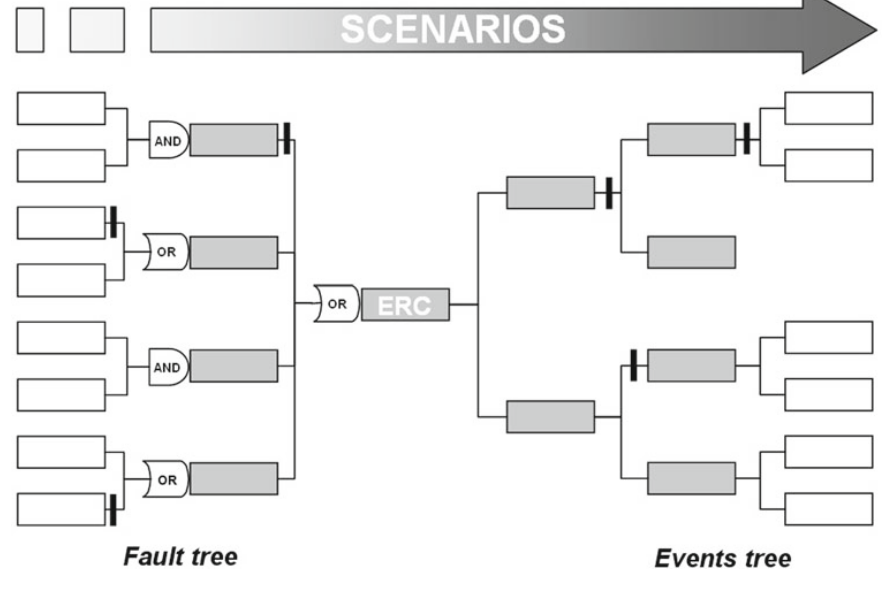
\includegraphics[width=0.5\linewidth]{figure/bowtie.png} 
  \caption{Gráfico de BowTie do texto \cite{melissaproject}}
  \label{bowtiegraf}
\end{figure}


Com o propósito de gerar reflexões no que tange aos riscos de dada atividade, o \textit{V3S} trabalha com o conceito de personagens virtuais em um ambiente. Os raciocínios a cerca destes personagens são feitos usando um formalismo matemático denominado por redes de Petri, ou - mais especificamente máquinas de estado \cite{v3sframework} tendo como base simular a complexidade, flexibilidade e variabilidade de comportamentos que podem ser verificados em um ser humano. Por conta disso, os cientistas desse estudo decidiram modelar esse comportamento usando sistemas multi-agentes, mas especificamente um \textit{framework} conhecido como MASVERP (tratado na seção \ref{agent}).

O \textit{V3S} tem como por finalidade providenciar um modelo que seja coerente, relevante, variado e eficiente em termos de cenário de treinamento com a finalidade de proporcionar atividades de aprendizagem. Esse modelo também apresenta um módulo que monitora cenários adaptativos conhecidos por \textit{HERA}.Em vez de interromper o usuário de forma sistemática a fim de explicar os erros dele, o framework possibilita que o agente cometa erros e observe suas respectivas consequências no mundo virtual. Portanto, a dinâmica do cenário adaptativo permite trazer situações de treinamento relevantes. 

\textit{HERA}, por intermédio de regras baseadas em modelos pedagógicos, fornece o respaldo ao instrutor. Esse retorno é feito por intermédio dos seguintes critérios pedagógicos; escala de modificação - amplia determinadas partes de um objeto com a finalidade de melhorar a visualização, reificação - verificar como o aprendiz lida com determinados conceitos e abstrações em termos concretos, restrições nos limites das ações do aprendiz que consiste em envio de mensagem ao agente quando ele comete sérios erros e superposição de informações se o aprendiz cometer e argumentar sobre as consequências das ações. \textit{HERA} é integrado ao módulo de reconhecimento que tem como por finalidade usar técnicas que permitem redefinir as relações de atividades usando a linguagem \textit{ACTIVITY-DL} se parametrizando nas açõe,s erros e violações. Essa parte do \textit{V3S} é capaz de distinguir entre os tipos de erros, que são: 1 - erros relacionados a atividades, 2 - erros relacionados ao ato de cumprir com o objetivo, 3 - erros de \textit{BATU}, 4 - erros de função e 5 - erros de ponto de vista.

De todos os modelos verificados neste estudo, o \textit{V3S} é o maior e o mais complexo abrangendo uma série de áreas que não está no escopo da representação em construção neste estudo. Isso não tira um potencial para análise comparativa sendo que o primeiro aspecto a ser verificado consiste numa análise sobre \textit{Domain Model} que define uma ontologia para representar todos os objetos, relações e ações. Sobre esse aspecto, ambos modelos possuem estruturas que se assemelham, mas a essa comparação é um tanto prejudicada tendo em vista que os termos usados em cada representação são diferentes. Outro ponto a ser considerado consiste no fato de que as verificações semânticas dos termos de \textit{Domain Model} não são claramente evidenciadas em \cite{v3sframework} e isso também ocasiona em uma dificuldade de comparação. 

Um dos termos presentes no \textit{V3S} é o \textit{V3S-Entity}. Esse vocábulo pode ser comparado, em partes, com o conjunto $ Entity $. A explicação disso se deve ao fato de que o \textit{V3S-Entity} possui uma relação denominada de \textit{is a} com a classe \textit{V3S-Object}. A relação \textit{is a} denota semanticamente que todo o elemento pertencente a \textit{V3S-Object} também é um elemento \textit{V3S-Entity} o que, na representação proposta neste estudo denota uma relação de herança "em termos de UML" ou uma relação de subconjunto $ \subset $. A figura presente em \ref{domainmodel} denota que o termo \textit{Valve} é um \textit{V3S-Object}. O termo \textit{Valve} que em português significa Válvula é algo que, para a representação que os pesquisadores desse estudo propõem, só pode ser definida como um artefato da classe $Artefact$. Logo, a relação $Artefact \subset Entity $ é equivalente a \textit{V3S-Object is a V3S-Entity}.

Os termos \textit{V3S-Object} $Artefact$ podem ser dados como semanticamente semelhantes (apesar de terem relações diferentes). Contudo o mesmo não pode ser feito para $Entity$ e \textit{V3S-Entity}, apesar do raciocínio presente no paragrafo anterior. Isso se deve ao fato de que \textit{V3S-Entity} não abrange os Agentes do modelo como é o caso de $Entity$. Outro ponto consiste na relação \textit{is a} entre \textit{V3S-Entity} com \textit{V3S-Action}. Antes se faz necessário verificar com qual termologia aquela expressão se assemelha no modelo proposto neste estudo. Para isso se faz necessário analisar a figura \ref{domainmodel} que apresenta \textit{Connect-On} como sendo um \textit{V3S-Action}, logo \textit{V3S-Entity}. É interessante observar que \textit{Connect-On} se relaciona tanto com o objeto \textit{Loading-Arm} bem como com objeto \textit{Valve}. Isso se assemelha em muito com o conceito de $Relation$ que tem como por finalidade representar a relação entre dois objetos. Dado essas proposições, é possível concluir que \textit{V3S-Action} é semalhante a $Relation$. Tendo em vista o fato que $Relation$ não é um subconjunto 
de $Entity$, isso denota que \textit{V3S-Entity} não é semanticamente semelhante a $Entity$. 

O segundo ponto a ser comparado reside sobre o modelo \textit{Activity Models} que basicamente consiste no uso da linguagem \textit{ACTIVITY-DL}. O que existe de equivalente a isso na representação proposta neste estudo são os objetivos descrito por $goal$ e o predicado $nextGoal(g_i,g_j)$ o que permite expressar raciocínios de eventos que podem acontecer tanto em série como em paralelo. Em contrapartida a isso, \textit{ACTIVITY-DL} permite expressar os seguintes racicínios; tarefas independentes, tarefas sequenciais, tarefas que se iniciam mediante a uma solicitação (pedido ou ordem), tarefas paralelas, tarefas  simultâneas, tarefas que se iniciam no mesmo instante e tarefas que são encerradas no mesmo instante. Portanto, em termos de relações entre tarefas o \textit{V3S} apresenta uma profundidade de representação muito maior quando comparado com o modelo proposto neste estudo. 

Parte das questões envolvendo erros, violações e risco tratadas no modelo proposto nesse estudo podem ser comparadas com aspectos da linguagem \textit{ACTIVITY-DL}. A concepção e análise de risco de ambos os modelos apresentam uma abordagem totalmente diferente, pois enquanto aquele faz uso de técnicas tal como \textit{BATUs} e \textit{BCTUs} para verificar atividades e condições que se apresentam dentro de um dado limite, este modelo não se preocupa em fazer uma descrição desse gênero das questões envolvendo segurança. Sobre certos aspectos existe uma certa semelhança pois relações de violação tanto de condições como de relações podem ser entendidas como o limite do razoável no qual o profissional deve agir. Sobre essa condição, as violações de condição estão para os \textit{BCTUs} e as violações de relações estão para os \textit{BATUs}. Contudo, é importante deixar evidente que ambas representações se fundamentam e apresentam estruturas de semânticas e de sintaxes completamente diferentes. 

O \textit{V3S} aprofunda as análises de segurança em \textit{Risk Model}. Essa parte do \textit{V3S} podem ser comparadas com as consequências que os riscos ocasionam sobre os agentes. Enquanto 
o \textit{V3S} faz uso de um \textit{framework} complexo denominado por MELISSA que tem como por finalidade tratar cenários de acidentes usando gráfico de \textit{Bowties}, o modelo proposto nesse estudo fornece um vocabulário relativamente mais simples e baseado nos conceitos de norma, violação e sanção presentes em estudos como o \cite{dastaniframework}. É interessante observar que muitos dos conceitos são os mesmos, tal como; riscos, consequências, relações de causalidades contudo os formalismos adotados são diferentes o que exprime raciocínios distintos. Por exemplo, situações onde um agente sofre consequências por algo que ele não fez podem ser especificadas com muito mais expressividade no estudo proposto neste trabalho do que no \textit{V3S}. O mesmo se dá na avaliação que vinculam a ocorrência dos acidentes em em relação aos artefatos e objetos presentes no ambiente. 

Um ponto interessante do \textit{Risk Model} consiste em uma representação MASVERP  de agente \textit{BDI} com o foco em Risco (ver em \ref{agent}). O modelo proposto neste estudo não trabalha com essa abordagem porque não é o foco delimitar a representação e o comportamento dos agentes.

Tanto este modelo como \textit{V3S} se preocupam em representar os mesmos cenários, gerar reflexões sobre as mesmas questões de definir e conduzir a uma análise de diversas condições existentes. Contudo, ambos os modelos adotam diferentes tipos de formalismos e articulam o vocabulário com aspectos distintos gerando diferenças bastante evidentes. Uma dessas diferenças reside na complexidade, sendo isso muito maior no \textit{V3S} que no modelo em proposta devido ao fato da quantidade de conceitos e de relações sobre as quais o modelador deverá refletir ao usar essas representações para o caso. Outro ponto reside na expressividade pois o \textit{V3S} apresenta maior grau disso nos seguintes aspectos; modelagem de atividade, condições limites onde os riscos são aceitáveis, cadeias de causalidades que resultam em acidentes, avaliação de questões didáticas e estados internos do agente. Já o modelo proposto neste estudo apresenta mais expressividade nos seguintes pontos; natureza dos erros cometidos pelos agentes em função das condições e componentes que estão presentes no ambiente, análise de como esses erros afetam a eles e a outros, análise de tipos de erros "violações" que ocasionam em consequências com natureza completamente diferente, consideração de questões estocásticas que afetam atividades de risco e o vínculo de todos os agentes, objetos e relações com os objetivos a serem atingidos. Outro aspecto que deve ser avaliado nessa comparação reside na metalinguagem usada para representar ambos modelos. A representação deste modelo adotou a teoria de conjuntos para escrever o modelo. Em contrapartida a isso, o \textit{V3S} está escrito em linguagem natural, formalismo usado para escrever ontologias e no formalismo usado para escrever algoritmos procedurais (talvez isso resida no fato de que o \textit{V3S} é conglomerado de outros modelos menores).